\usepackage{noweb}
\noweboptions{smallcode,longchunks,longxref}

\usepackage[T1]{fontenc}
%\usepackage{imfellEnglish}
%\usepackage[default]{gillius}
\usepackage{CormorantGaramond}
%\usepackage[el,nf]{coelacanth}
\usepackage[zerostyle=d]{newtxtt}
%\usepackage{FiraMono}

\usepackage[utf8]{inputenc}
% \usepackage[french]{babel}

\usepackage{xcolor}
\usepackage{tikz}

\definecolor{mygray}{rgb}{0.4,0.4,0.4}
\usepackage[bookmarks,backref=page,linkcolor=mygray]{hyperref} %,colorlinks
\hypersetup{%
  pdfauthor = {Bernard Tatin},
  pdftitle = {},
  pdfsubject = {},
  pdfkeywords = {},
  colorlinks=true,
  linkcolor= mygray,
  citecolor= black,
  pageanchor=true,
  urlcolor = mygray,
  plainpages = false,
  linktocpage
}

\let\oldabstract\abstract
\renewenvironment{abstract}[1]{%
  \hfill
  \begin{minipage}
    {0.95\textwidth}
    \rule{\textwidth}{1pt}
    \footnotesize
    #1
    \normalsize
    {%
      \par\noindent
      \rule{\textwidth}{1pt}
    }
  \end{minipage}
}
%% format des paragraphes
%% \setlength{\parindent}{0cm}
%% \setlength{\parskip}{4mm}
%% \linespread{1.1}
%% \let\nwdocspar=\smallbreak

\newenvironment{packed_itemize}{
\begin{itemize}
  \setlength{\itemsep}{0pt}
  \setlength{\parskip}{0pt}
  \setlength{\parsep}{0pt}
}{\end{itemize}}

%
%
\setkomafont{section}{\color{mygray}%
  \bfseries\Large
  
\begin{tikzpicture}[overlay]
  \draw[fill=orange] (0,-5pt) rectangle
  (\linewidth,16.4pt);
  \end{tikzpicture}}
\setkomafont{subsection}{\color{black}%
  \itshape\bfseries\large
  \begin{tikzpicture}[overlay]
  \draw[fill=yellow] (0,-5pt) rectangle
  (\linewidth,16.4pt);
  \end{tikzpicture}}
\setkomafont{subsubsection}{\color{mygray}%
  \itshape\normalsize
  \begin{tikzpicture}[overlay]
  \draw[fill=yellow] (0,-5pt) rectangle
  (\linewidth,16.4pt);
  \end{tikzpicture}}
